\documentclass{standalone}
\usepackage{tikz}
\usetikzlibrary{patterns, positioning}
\usepackage[sfdefault]{ClearSans} %% option 'sfdefault' activates Clear Sans as the default text font
\usepackage[T1]{fontenc}

\begin{document}
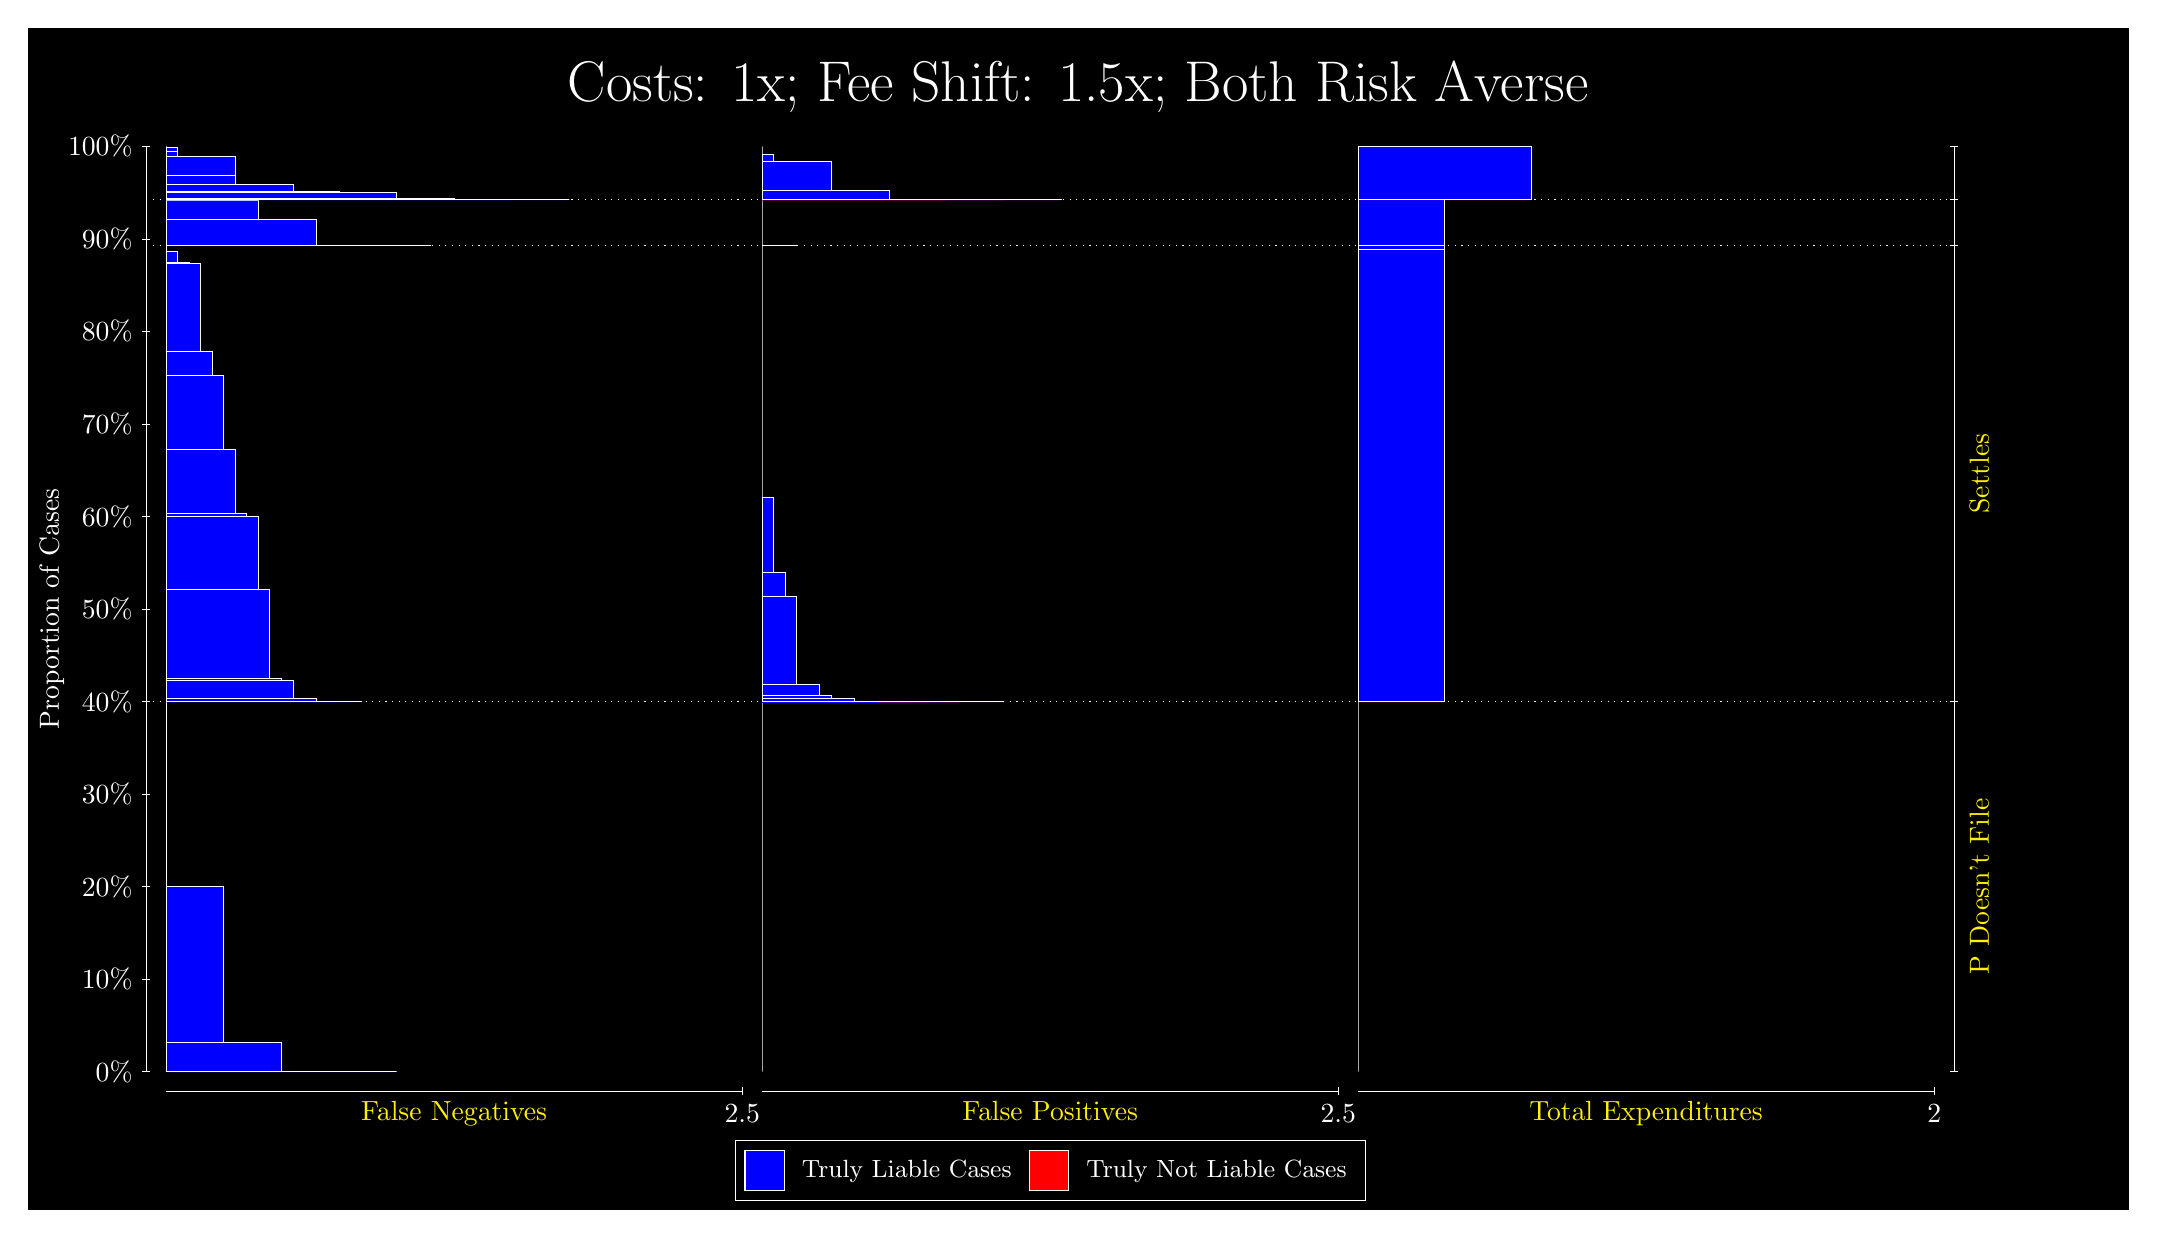
\begin{tikzpicture}
\draw[fill=black] (0,0) rectangle (26.667,15);
\draw[text=white] (0,13.5) rectangle (26.667,15) node[midway] {\huge Costs: 1x; Fee Shift: 1.5x; Both Risk Averse};
\draw[white, very thin] (1.5,1.75) -- (1.5,13.5);
\node[rotate=90, text=white, anchor=center] at (0.3, 7.625) {Proportion of Cases};
\draw[white, very thin] (1.45,1.75) -- (1.55,1.75);
\node[text=white, anchor=east] at (1.45, 1.75) {0\%};
\draw[white, very thin] (1.45,2.925) -- (1.55,2.925);
\node[text=white, anchor=east] at (1.45, 2.925) {10\%};
\draw[white, very thin] (1.45,4.1) -- (1.55,4.1);
\node[text=white, anchor=east] at (1.45, 4.1) {20\%};
\draw[white, very thin] (1.45,5.275) -- (1.55,5.275);
\node[text=white, anchor=east] at (1.45, 5.275) {30\%};
\draw[white, very thin] (1.45,6.45) -- (1.55,6.45);
\node[text=white, anchor=east] at (1.45, 6.45) {40\%};
\draw[white, very thin] (1.45,7.625) -- (1.55,7.625);
\node[text=white, anchor=east] at (1.45, 7.625) {50\%};
\draw[white, very thin] (1.45,8.8) -- (1.55,8.8);
\node[text=white, anchor=east] at (1.45, 8.8) {60\%};
\draw[white, very thin] (1.45,9.975) -- (1.55,9.975);
\node[text=white, anchor=east] at (1.45, 9.975) {70\%};
\draw[white, very thin] (1.45,11.15) -- (1.55,11.15);
\node[text=white, anchor=east] at (1.45, 11.15) {80\%};
\draw[white, very thin] (1.45,12.325) -- (1.55,12.325);
\node[text=white, anchor=east] at (1.45, 12.325) {90\%};
\draw[white, very thin] (1.45,13.5) -- (1.55,13.5);
\node[text=white, anchor=east] at (1.45, 13.5) {100\%};

\draw[white, very thin] (24.457,1.75) -- (24.457,13.5);
\draw[white, very thin] (24.407,1.75) -- (24.507,1.75);
\node[anchor=west] at (24.407, 1.75) {};
\draw[white, very thin] (24.407,6.4489) -- (24.507,6.4489);
\node[anchor=west] at (24.407, 6.4489) {};
\draw[white, very thin] (24.407,12.241) -- (24.507,12.241);
\node[anchor=west] at (24.407, 12.241) {};
\draw[white, very thin] (24.407,12.823) -- (24.507,12.823);
\node[anchor=west] at (24.407, 12.823) {};
\draw[white, very thin] (24.407,13.5) -- (24.507,13.5);
\node[anchor=west] at (24.407, 13.5) {};

\draw[white, very thin, fill=blue] (1.75,1.75) rectangle (4.6775,1.75);
\draw[white, very thin, fill=blue] (1.75,1.75) rectangle (3.9457,1.7532);
\draw[white, very thin, fill=blue] (1.75,1.7532) rectangle (3.2138,2.126);
\draw[white, very thin, fill=blue] (1.75,2.126) rectangle (2.4819,4.1027);
\draw[white, very thin, fill=red] (1.75,4.1027) rectangle (1.75,4.1027);
\draw[white, very thin, fill=blue] (1.75,4.1027) rectangle (1.75,6.4489);
\draw[white, very thin, fill=blue] (1.75,6.4489) rectangle (4.2384,6.4489);
\draw[white, very thin, fill=blue] (1.75,6.4489) rectangle (3.9457,6.449);
\draw[white, very thin, fill=blue] (1.75,6.449) rectangle (3.6529,6.4913);
\draw[white, very thin, fill=blue] (1.75,6.4913) rectangle (3.5065,6.493);
\draw[white, very thin, fill=blue] (1.75,6.493) rectangle (3.3602,6.7141);
\draw[white, very thin, fill=blue] (1.75,6.7141) rectangle (3.2138,6.7433);
\draw[white, very thin, fill=blue] (1.75,6.7433) rectangle (3.0674,7.8747);
\draw[white, very thin, fill=blue] (1.75,7.8747) rectangle (2.921,8.8039);
\draw[white, very thin, fill=blue] (1.75,8.8039) rectangle (2.7746,8.8408);
\draw[white, very thin, fill=blue] (1.75,8.8408) rectangle (2.6283,9.651);
\draw[white, very thin, fill=blue] (1.75,9.651) rectangle (2.4819,10.597);
\draw[white, very thin, fill=blue] (1.75,10.597) rectangle (2.3355,10.903);
\draw[white, very thin, fill=blue] (1.75,10.903) rectangle (2.1891,12.019);
\draw[white, very thin, fill=blue] (1.75,12.019) rectangle (2.0428,12.026);
\draw[white, very thin, fill=blue] (1.75,12.026) rectangle (1.8964,12.161);
\draw[white, very thin, fill=red] (1.75,12.161) rectangle (1.75,12.161);
\draw[white, very thin, fill=blue] (1.75,12.161) rectangle (1.75,12.241);
\draw[white, very thin, fill=blue] (1.75,12.241) rectangle (5.1167,12.241);
\draw[white, very thin, fill=blue] (1.75,12.241) rectangle (4.3848,12.248);
\draw[white, very thin, fill=blue] (1.75,12.248) rectangle (3.6529,12.569);
\draw[white, very thin, fill=blue] (1.75,12.569) rectangle (2.921,12.82);
\draw[white, very thin, fill=blue] (1.75,12.82) rectangle (2.1891,12.823);
\draw[white, very thin, fill=red] (1.75,12.823) rectangle (1.75,12.823);
\draw[white, very thin, fill=blue] (1.75,12.823) rectangle (6.8732,12.823);
\draw[white, very thin, fill=blue] (1.75,12.823) rectangle (6.1413,12.823);
\draw[white, very thin, fill=blue] (1.75,12.823) rectangle (5.4094,12.838);
\draw[white, very thin, fill=blue] (1.75,12.838) rectangle (4.8239,12.838);
\draw[white, very thin, fill=blue] (1.75,12.838) rectangle (4.6775,12.917);
\draw[white, very thin, fill=blue] (1.75,12.917) rectangle (4.092,12.917);
\draw[white, very thin, fill=blue] (1.75,12.917) rectangle (3.9457,12.923);
\draw[white, very thin, fill=blue] (1.75,12.923) rectangle (3.3602,13.015);
\draw[white, very thin, fill=blue] (1.75,13.015) rectangle (3.2138,13.015);
\draw[white, very thin, fill=blue] (1.75,13.015) rectangle (2.6283,13.135);
\draw[white, very thin, fill=blue] (1.75,13.135) rectangle (2.6283,13.379);
\draw[white, very thin, fill=blue] (1.75,13.379) rectangle (2.4819,13.379);
\draw[white, very thin, fill=blue] (1.75,13.379) rectangle (1.8964,13.434);
\draw[white, very thin, fill=blue] (1.75,13.434) rectangle (1.8964,13.494);
\draw[white, very thin, fill=red] (1.75,13.494) rectangle (1.75,13.494);
\draw[white, very thin, fill=blue] (1.75,13.494) rectangle (1.75,13.5);
\draw[white, very thin, fill=red] (9.3189,1.75) rectangle (9.3189,1.75);
\draw[white, very thin, fill=blue] (9.3189,1.75) rectangle (9.3189,6.4489);
\draw[white, very thin, fill=red] (9.3189,6.4489) rectangle (12.393,6.4489);
\draw[white, very thin, fill=blue] (9.3189,6.4489) rectangle (12.393,6.4489);
\draw[white, very thin, fill=red] (9.3189,6.4489) rectangle (11.807,6.4489);
\draw[white, very thin, fill=blue] (9.3189,6.4489) rectangle (11.807,6.4489);
\draw[white, very thin, fill=blue] (9.3189,6.4489) rectangle (11.661,6.4489);
\draw[white, very thin, fill=red] (9.3189,6.4489) rectangle (11.515,6.4489);
\draw[white, very thin, fill=blue] (9.3189,6.4489) rectangle (11.515,6.4489);
\draw[white, very thin, fill=red] (9.3189,6.4489) rectangle (11.222,6.4489);
\draw[white, very thin, fill=blue] (9.3189,6.4489) rectangle (11.222,6.4489);
\draw[white, very thin, fill=blue] (9.3189,6.4489) rectangle (11.075,6.4489);
\draw[white, very thin, fill=red] (9.3189,6.4489) rectangle (10.929,6.4489);
\draw[white, very thin, fill=blue] (9.3189,6.4489) rectangle (10.929,6.4489);
\draw[white, very thin, fill=blue] (9.3189,6.4489) rectangle (10.783,6.4492);
\draw[white, very thin, fill=red] (9.3189,6.4492) rectangle (10.636,6.4492);
\draw[white, very thin, fill=blue] (9.3189,6.4492) rectangle (10.636,6.4492);
\draw[white, very thin, fill=blue] (9.3189,6.4492) rectangle (10.49,6.4899);
\draw[white, very thin, fill=blue] (9.3189,6.4899) rectangle (10.344,6.4913);
\draw[white, very thin, fill=blue] (9.3189,6.4913) rectangle (10.197,6.5285);
\draw[white, very thin, fill=blue] (9.3189,6.5285) rectangle (10.051,6.664);
\draw[white, very thin, fill=blue] (9.3189,6.664) rectangle (9.9044,6.6709);
\draw[white, very thin, fill=blue] (9.3189,6.6709) rectangle (9.758,7.7868);
\draw[white, very thin, fill=blue] (9.3189,7.7868) rectangle (9.6116,8.0932);
\draw[white, very thin, fill=blue] (9.3189,8.0932) rectangle (9.4652,9.0388);
\draw[white, very thin, fill=blue] (9.3189,9.0388) rectangle (9.3189,12.241);
\draw[white, very thin, fill=red] (9.3189,12.241) rectangle (9.758,12.241);
\draw[white, very thin, fill=blue] (9.3189,12.241) rectangle (9.758,12.244);
\draw[white, very thin, fill=blue] (9.3189,12.244) rectangle (9.3189,12.823);
\draw[white, very thin, fill=red] (9.3189,12.823) rectangle (13.125,12.823);
\draw[white, very thin, fill=blue] (9.3189,12.823) rectangle (13.125,12.823);
\draw[white, very thin, fill=red] (9.3189,12.823) rectangle (12.393,12.823);
\draw[white, very thin, fill=blue] (9.3189,12.823) rectangle (12.393,12.823);
\draw[white, very thin, fill=red] (9.3189,12.823) rectangle (11.661,12.823);
\draw[white, very thin, fill=blue] (9.3189,12.823) rectangle (11.661,12.829);
\draw[white, very thin, fill=red] (9.3189,12.829) rectangle (10.929,12.829);
\draw[white, very thin, fill=blue] (9.3189,12.829) rectangle (10.929,12.945);
\draw[white, very thin, fill=red] (9.3189,12.945) rectangle (10.344,12.945);
\draw[white, very thin, fill=blue] (9.3189,12.945) rectangle (10.344,12.945);
\draw[white, very thin, fill=blue] (9.3189,12.945) rectangle (10.197,13.308);
\draw[white, very thin, fill=red] (9.3189,13.308) rectangle (9.6116,13.308);
\draw[white, very thin, fill=blue] (9.3189,13.308) rectangle (9.6116,13.308);
\draw[white, very thin, fill=blue] (9.3189,13.308) rectangle (9.4652,13.4);
\draw[white, very thin, fill=red] (9.3189,13.4) rectangle (9.3189,13.4);
\draw[white, very thin, fill=blue] (9.3189,13.4) rectangle (9.3189,13.5);
\draw[white, very thin, fill=red] (16.888,1.75) rectangle (16.888,1.75);
\draw[white, very thin, fill=blue] (16.888,1.75) rectangle (16.888,6.4489);
\draw[white, very thin, fill=red] (16.888,6.4489) rectangle (17.986,6.4489);
\draw[white, very thin, fill=blue] (16.888,6.4489) rectangle (17.986,12.195);
\draw[white, very thin, fill=red] (16.888,12.195) rectangle (17.986,12.195);
\draw[white, very thin, fill=blue] (16.888,12.195) rectangle (17.986,12.241);
\draw[white, very thin, fill=red] (16.888,12.241) rectangle (17.986,12.241);
\draw[white, very thin, fill=blue] (16.888,12.241) rectangle (17.986,12.823);
\draw[white, very thin, fill=red] (16.888,12.823) rectangle (19.083,12.823);
\draw[white, very thin, fill=blue] (16.888,12.823) rectangle (19.083,13.5);
\draw[white, dotted] (1.5,6.4489) -- (24.457,6.4489);
\draw[white, dotted] (1.5,12.241) -- (24.457,12.241);
\draw[white, dotted] (1.5,12.823) -- (24.457,12.823);
\draw[white, very thin] (1.75,1.5) -- (9.0689,1.5);
\node[text=yellow, anchor=north] at (5.4094, 1.5) {False Negatives};
\draw[white, very thin] (9.0689,1.45) -- (9.0689,1.55);
\node[text=white, anchor=north] at (9.0689, 1.45) {2.5};

\draw[white, very thin] (9.3189,1.5) -- (16.638,1.5);
\node[text=yellow, anchor=north] at (12.978, 1.5) {False Positives};
\draw[white, very thin] (16.638,1.45) -- (16.638,1.55);
\node[text=white, anchor=north] at (16.638, 1.45) {2.5};

\draw[white, very thin] (16.888,1.5) -- (24.207,1.5);
\node[text=yellow, anchor=north] at (20.547, 1.5) {Total Expenditures};
\draw[white, very thin] (24.207,1.45) -- (24.207,1.55);
\node[text=white, anchor=north] at (24.207, 1.45) {2};

\node[text=yellow, centered, rotate=90] at (24.777, 4.0995) {P Doesn't File};
\node[text=yellow, centered, rotate=90] at (24.777, 9.3449) {Settles};



\draw (12.978300999999998,1.5) node[draw=none] (baseCoordinate) {};
\begin{scope}[align=center]
        \matrix[scale=0.5, draw=white, below=0.5cm of baseCoordinate, nodes={draw}, column sep=0.1cm]{
            \node[rectangle, draw, minimum width=0.5cm, minimum height=0.5cm, fill=blue] {}; &
            \node[draw=none, font=\small, text=white] (B) {Truly Liable Cases}; &
            \node[rectangle, draw, minimum width=0.5cm, minimum height=0.5cm, fill=red] {}; &
            \node[draw=none, font=\small, text=white] (B) {Truly Not Liable Cases}; \\
            };
\end{scope}

\end{tikzpicture}
\end{document}